\section{Parameter identification}
\label{SubSecEstimation}

The behavior of the complete water distribution system is governed by the previously derived model, however certain parameters of the system are either unknown or can vary significantly from the assumed design values. Furthermore, the obtained model of the system gives non-linear relations between flows and pressures in each individual components. 
\\
In case of the valves, the conductivity function is dependant on the OD, therefore the parameter of these elements are considered to be known. The centrifugal pumps are fully described by their models and by the coefficients provided by the manufacturer. The hydraulic capacity is also considered as known in case of the WT. However, certain parameters in the model of pipes are uncertain. Even though the necessary friction parameters can be found in the data sheet provided by the manufacturer, these values are only acceptable for new pipes, as over time material can build up on the inside of the pipes, since the laboratory set up to a large extent is built from PEX/PEM (plastic) pipes. On the other hand however, the physical parameters of the pipe volumes are assumed to be known to an accuracy where there is not any benefits from estimating it. Therefore the inertia matrix is known.  
\\
Consequently, the aim of the system identification in case of the water distribution system is to estimate the missing parameters which describe the frictions and form losses(which cause the major uncertainty in this case) in the pipes, therefore define the additional pressure losses. Due to these considerations, the importance of obtaining accurate parameters is essential in order to set up a simulation that represents the real test set up. 

The parameter estimation is introduced for two different cases with different approaches. One being an estimation method with the model being kept non-linear, the other being a method where the model is  linearized before the estimation. 

The block diagram of a general parameter identification method is described in \figref{fig:parame_block} below: 

\begin{figure}[H]
\centering
\usetikzlibrary{arrows}
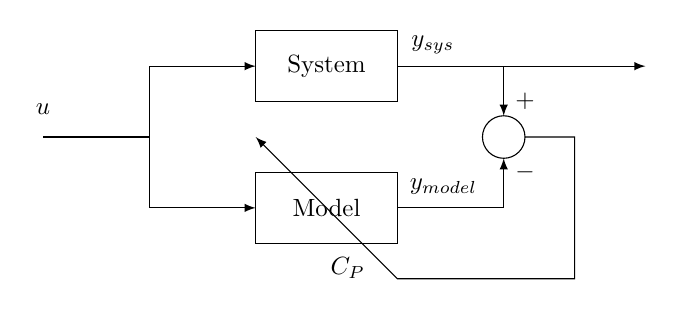
\begin{tikzpicture} [scale=0.9,transform shape]

\draw  (3,-1.5) rectangle (5,-2.5);
\node at (4,-2) {Model};

\draw  (3,0.5) rectangle (5,-0.5);
\node at (4,0) {System};

\node at (6.8,-1.5) {$-$};
\node at (5.5,0.3) {$y_{sys}$};
\node at (5.65,-1.7) {$y_{model}$};
\node at (4.3,-2.85) {$C_P$};
\node at (0,-0.6) {$u$};
\node at (6.8,-0.5) {$+$};

\draw  (6.5,-1) ellipse (0.3 and 0.3);

\draw [-latex](5,0) -- (8.5,0);
\draw [-latex](6.5,0) -- (6.5,-0.7);
\draw [-latex](1.5,-1) -- (1.5,0) -- (3,0);
\draw [-latex](1.5,-1) -- (1.5,-2) -- (3,-2);
\draw (0,-1) -- (1.5,-1);
\draw [-latex](5,-2) -- (6.5,-2) -- (6.5,-1.3);
\draw [-latex](6.8,-1) -- (7.5,-1) -- (7.5,-3) -- (5,-3) -- (3,-1);

\end{tikzpicture}% 
\caption{Parameter identification block diagram. }
\label{fig:parame_block}
\end{figure}

As it is shown in the figure, the measurements from the real life system are compared to the output of the simulation. In general, the inputs are the same for both systems, however some modifications have to be introduced in the case of the linearized model. (This is explained in detail in the section covering the linear parameter identification method.)
\\
In order to obtain measurements from the real life test set up, the system has to be excited by various input signals. In general, the inputs to the system are the input signals to the pumps, however in case of the parameter estimation the OD of the valves is also considered as an input. Therefore it is reasonable to reformulate the equation describing the network in \eqref{ParatModelFinal} into such a form where the expressions for the inputs and states are isolated. Such an expression can be obtained for the whole network from the general model as follows: 

\begin{equation}
 \pmb{B}\pmb{J {B}}^T \pmb{\dot{z}} = \pmb{B} g(\pmb{B}^T \pmb{z})+ \pmb{B} u(\pmb{\omega},\pmb{k_v	}, \pmb{B}^T \pmb{z})
 \label{InputOutputmodel}
\end{equation}

where the vectorfield $u(.)$ contains all the functions for the elements which are dependant on the inputs and the vectorfield $g(.)$ describes the rest of the resistance terms which are responsible for the pressure drops in any part of the network. Although $u(.)$ is a function of $\omega$ and $k_v$, in the simulation however the inputs to the pumps are specified as pressure differences, $dp$, because the value of these pressures are available on the test set up. 
\\
In the system, output are defined as differential pressures according to the available sensors on the test set up. From the system setup $8$ different relative pressures can be measured. Following the notation of \figref{systemdiagram}, sensors are placed in: 
$n_2$ $n_4$ $n_5$ $n_7$ $n_{10}$ $n_{11}$ $n_{15}$ $n_{16}$. During the parameter identification, these measurements are compared to the output from the simulation and the parameters are varied until they fit.
\\
It is important to point out that the estimation is applied for steady-state which is reasonable, since the unknown parameters are the resistances and form losses and the inertia and the capacitance only affect the dynamics, therefore have no influence on the steady-state. The inertia of the pipes, and the capacitance of the WT is considered as known parameters. 

Taking the steady-state into account, the system equation for the parameter estimation can be rewritten as: 

\begin{equation}
 0 = \pmb{B} g(\pmb{B}^T \pmb{z})+ \pmb{B} u(\pmb{\omega},\pmb{k_v}, \pmb{B}^T \pmb{z})
 \label{InputOutputmodel_steadystate}
\end{equation}

The aim of the parameter identification is therefore to obtain a minimum difference between the outputs by adjusting the parameters of the model. (The number of parameters are equal to the number of pipe elements in the network.) The general parameter estimation problem is the problem of the minimization of the following objective function over the variable $\pmb{z}$: 

%\begin{equation}
%
%  \sum_{i=1}^{n}\Big(g_{\pmb(Cp)}(\pmb{B}^T \pmb{z}_i)\Big)
%
%\label{ObjectiveFunction}
%\end{equation}

 \begin{equation}
 \min_{z} \sum_{i=1}^{n}\Big(g(z_i) + B_i^Tu_i\Big)^T \Big(g(z_i)     + B_i^Tu_i\Big) + \big(y_{sys;i} - y(z_i)\big)^T  \big(y_{sys;i} - y(z_i)\big)
  \label{ObjectiveFunction}
 \end{equation}
 
\begin{minipage}[t]{0.20\textwidth}
Where\\
\hspace*{8mm} $n$ \\
\hspace*{8mm} $g(z_i)$ \\
\hspace*{8mm} $u$ \\
\hspace*{8mm} $y_{sys;i}$ \\
\hspace*{8mm} $y_{sys}(z_i)$ 
\end{minipage}
\begin{minipage}[t]{0.68\textwidth}
\vspace*{2mm}
is the number of edges in the graph-based network,\\
is the vectorfield with all resistance terms(parameters),\\
is the vectorfield with the inputs,\\
is the pressure measurement over the $i^{th}$ edge on the system,\\
is the $i^{th}$ pressure in the output vector in the model .
\end{minipage}
\begin{minipage}[t]{0.10\textwidth}
\vspace*{2mm}
\textcolor{White}{te}$\unit{-}$
\textcolor{White}{te}$\unit{bar}$
\textcolor{White}{te}$\unit{bar}$
\textcolor{White}{te}$\unit{bar}$
\textcolor{White}{te}$\unit{bar}$
\end{minipage}

 





%Applying KVL to the hydraulic model, the following expression is obtained: Moreover, the parameter estimation is carried out for steady-state 
%situation where the inertia, $J$, will not act. Thus, the term containing the diagonal matrix $J$ can be disregarded from the equation. 
%
%\begin{equation}
%  0 = \pmb{B_1 \Delta p_1 }= \pmb{B_1} [ \pmb{J {B_1}}^T \pmb{\dot{z}} + f(\pmb{z},\pmb{ w}, \pmb{k_v})]  = \pmb{ B_1} (f(\pmb{z}, \pmb{w},\pmb{ k_v}))
%  \label{esteq}
% \end{equation}
 
%The pressure difference in the pumps have been specified as inputs, by reason of those pressures can be obtained from the setup available so they are considered 
%as known parameters. Thereby, in \eqref{esteq} the term can be split up as following:
% 
%\begin{equation}
% 0 = f(\pmb{z},\pmb{k_v})+ f(\pmb{z},\pmb{w})
% \label{ModelNoInertia}
%\end{equation}

%The term $f(\pmb{z},\pmb{w})$ is set as input, it is renamed as U and it represents the pressure difference in the $4$ pumps acting on the system. Therefore, 
%\eqref{ModelNoInertia} is considered as the input equation where the flow through the chords and the friction parameter of the pipes are unknown. 
%
%An output equation is defined, which represents the pressure difference known from the system setup. In this way, the output equation can be compared 
%to the data measured in the setup and proceed to estimate the unknown parameters. 

%From the system setup $8$ different relative pressures can be measured, following \figref{systemdiagram} notation the sensors are placed in: 
%$n_2$ $n_4$ $n_5$ $n_7$ $n_{10}$ $n_{11}$ $n_{15}$ $n_{16}$.

%In order to compare the measurements from the system setup and the data obtained from the simulation in Matlab, a reference point has to be set in the 
%simulation to calculate the desired data. 
%
%The atmospheric is set as reference point and the pressures obtained from the simulation are dependant on it. The relationship between pressures, where DpCXX describes
%the pressure difference for the XX component, can be defined as:
%
%\text{\underline{Node 2}} 
%\vspace{4mm}
%\begin{equation}
%    DpC2 = y_1
%\end{equation}
%
%\text{\underline{Node 7}}
%\vspace{4mm}
%\begin{equation}
%  DpC16 = y_2
%\end{equation}
%
%\text{\underline{Node 4}}
%\vspace{4mm}
%\begin {equation}
%    DpC18 + DpC19 + DpC23 + DpC24 = y_3
%\end{equation}
%
%\text{\underline{Node 5}}
%\vspace{4mm}
%\begin {equation}
%    DpC25 + DpC26 + DpC30 + DpC31 = y_4
%\end{equation}
%
%\text{\underline{Node 10}}
%\vspace{4mm}
%\begin {equation}
%    DpC24 = y_5
%\end{equation}
%
%\text{\underline{Node 11}}
%\vspace{4mm}
%\begin {equation}
%    DpC20 + DpC21= y_6
%\end{equation}
%
%\text{\underline{Node 15}}
%\vspace{4mm}
%\begin {equation}
%    DpC31 = y_7
%\end{equation}
%
%\text{\underline{Node 16}}
%\vspace{4mm}
%\begin {equation}
%    DpC28 + DpC27 = y_8
%\end{equation}
%
%
%With the $8$ equations depicted above the output vector $\pmb{y}$ is obtained. 